\documentclass{beamer}
\mode<presentation>
%% \mode<handout>{\setbeamercolor{background canvas}{bg=black!5}}
\usetheme{CambridgeUS}
\usecolortheme{dolphin}

\usepackage{bstyle}
\usepackage{bibentry}

\renewcommand{\footnotesize}{\scriptsize}

\title[]{Searching in the Space of Persistence Diagrams}

\author{
        Samuel Micka\thanks{School of Computing,
            Montana State
            U. }
    }
\index{Micka, Samuel}
\date[5 April 2019]{April 5th, 2019}

\begin{document}
\begin{frame}
\titlepage
\centering
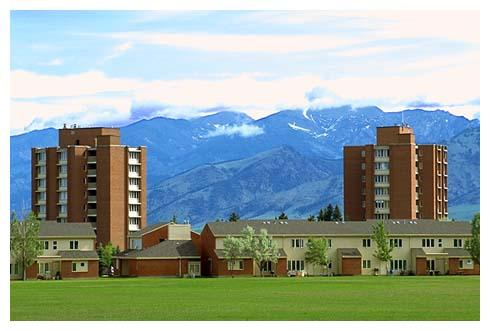
\includegraphics[width=.5\textwidth]{figs/msu}
\bibliographystyle{acm}
\nobibliography{references}
\end{frame}

\frame{
    \frametitle{Samuel Micka}
\begin{block}{About Me}
\centering
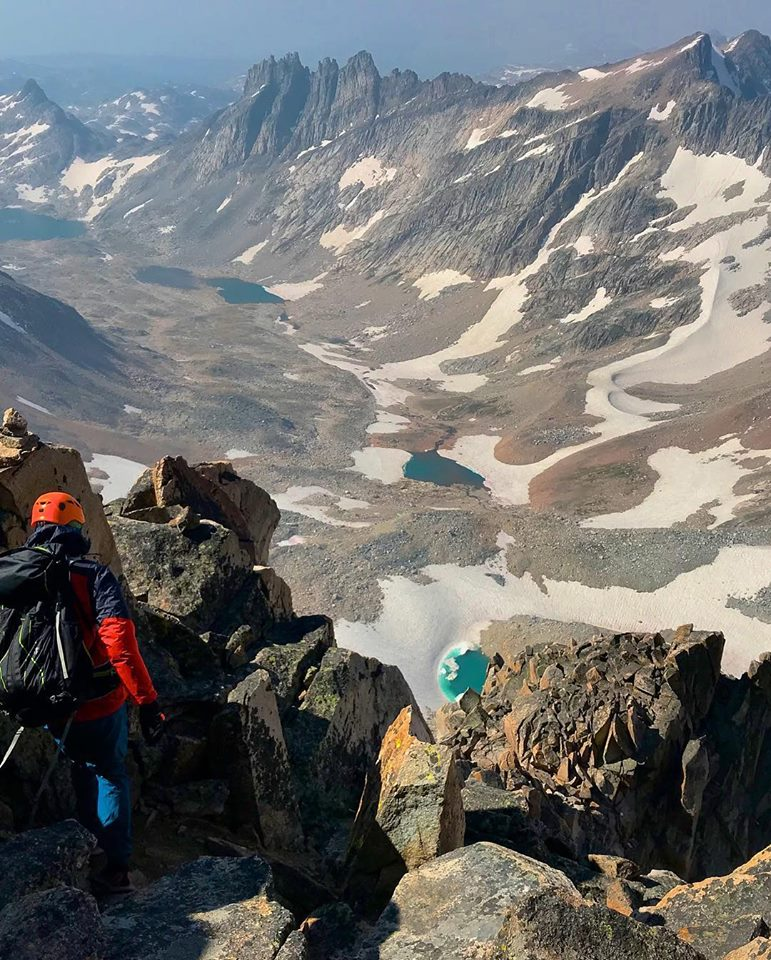
\includegraphics[height=30mm]{figs/granite-sam}\hspace{5mm}
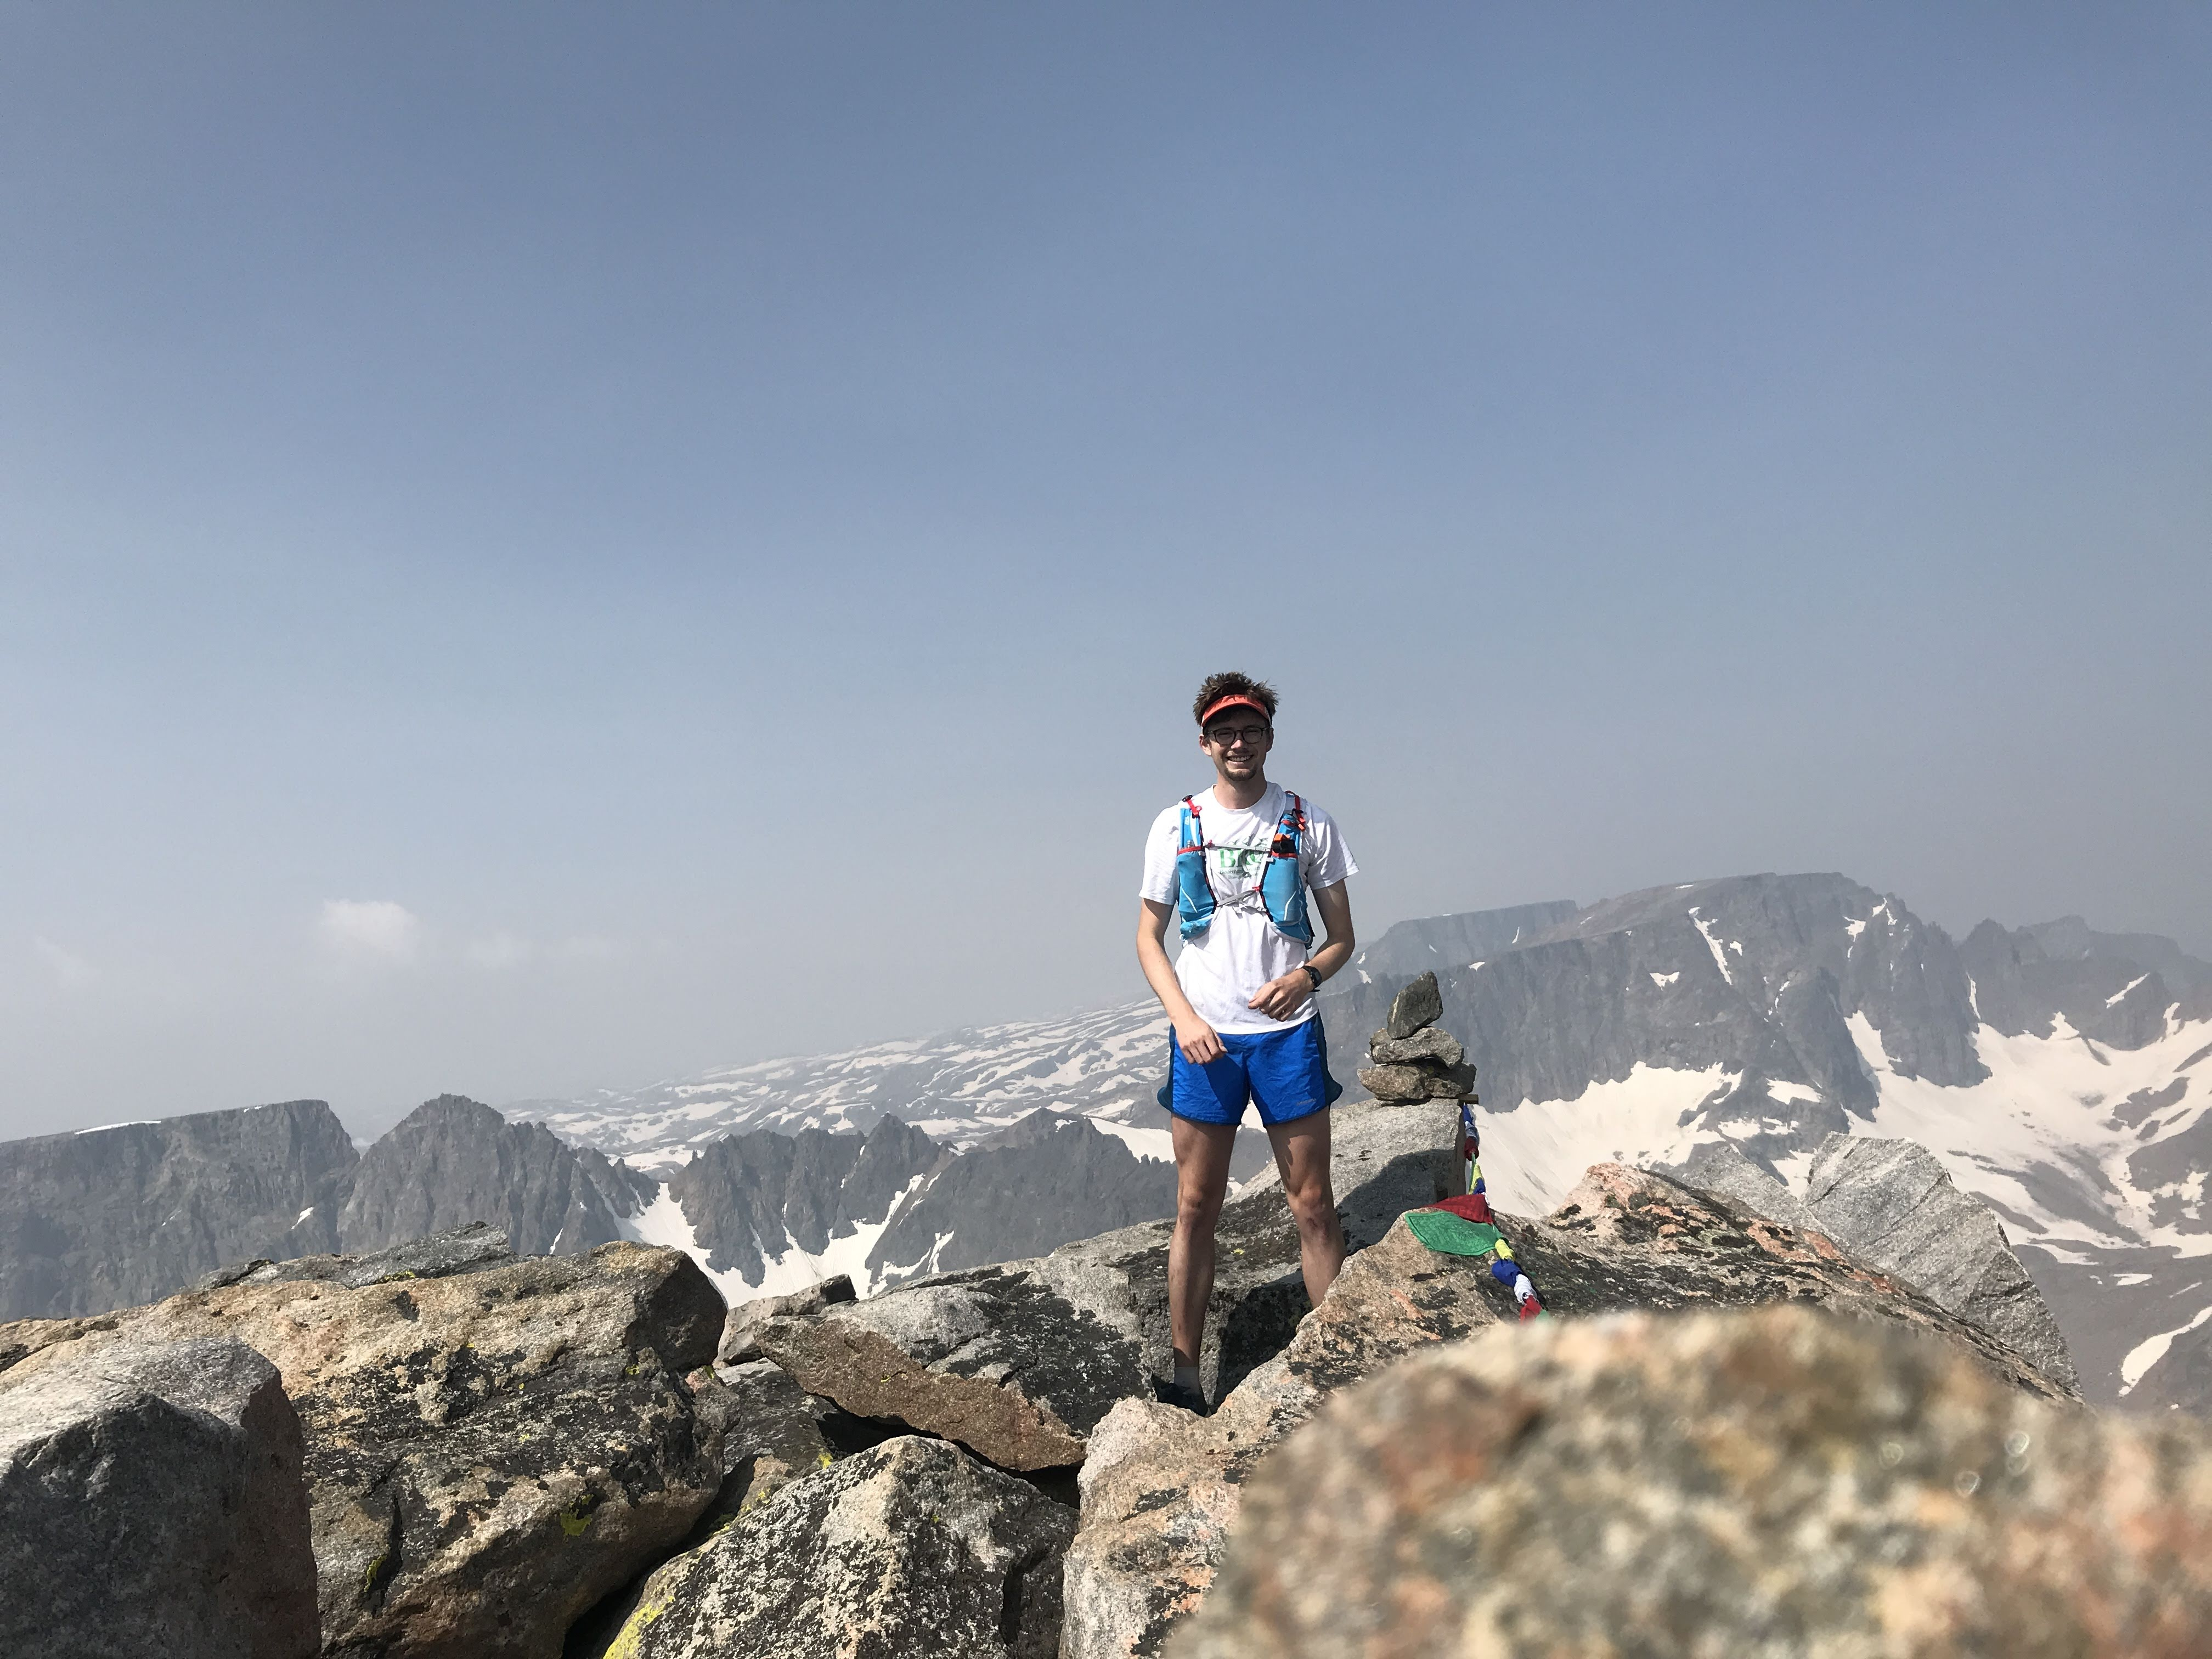
\includegraphics[height=30mm]{figs/whitetail}\\
\vspace{5mm}
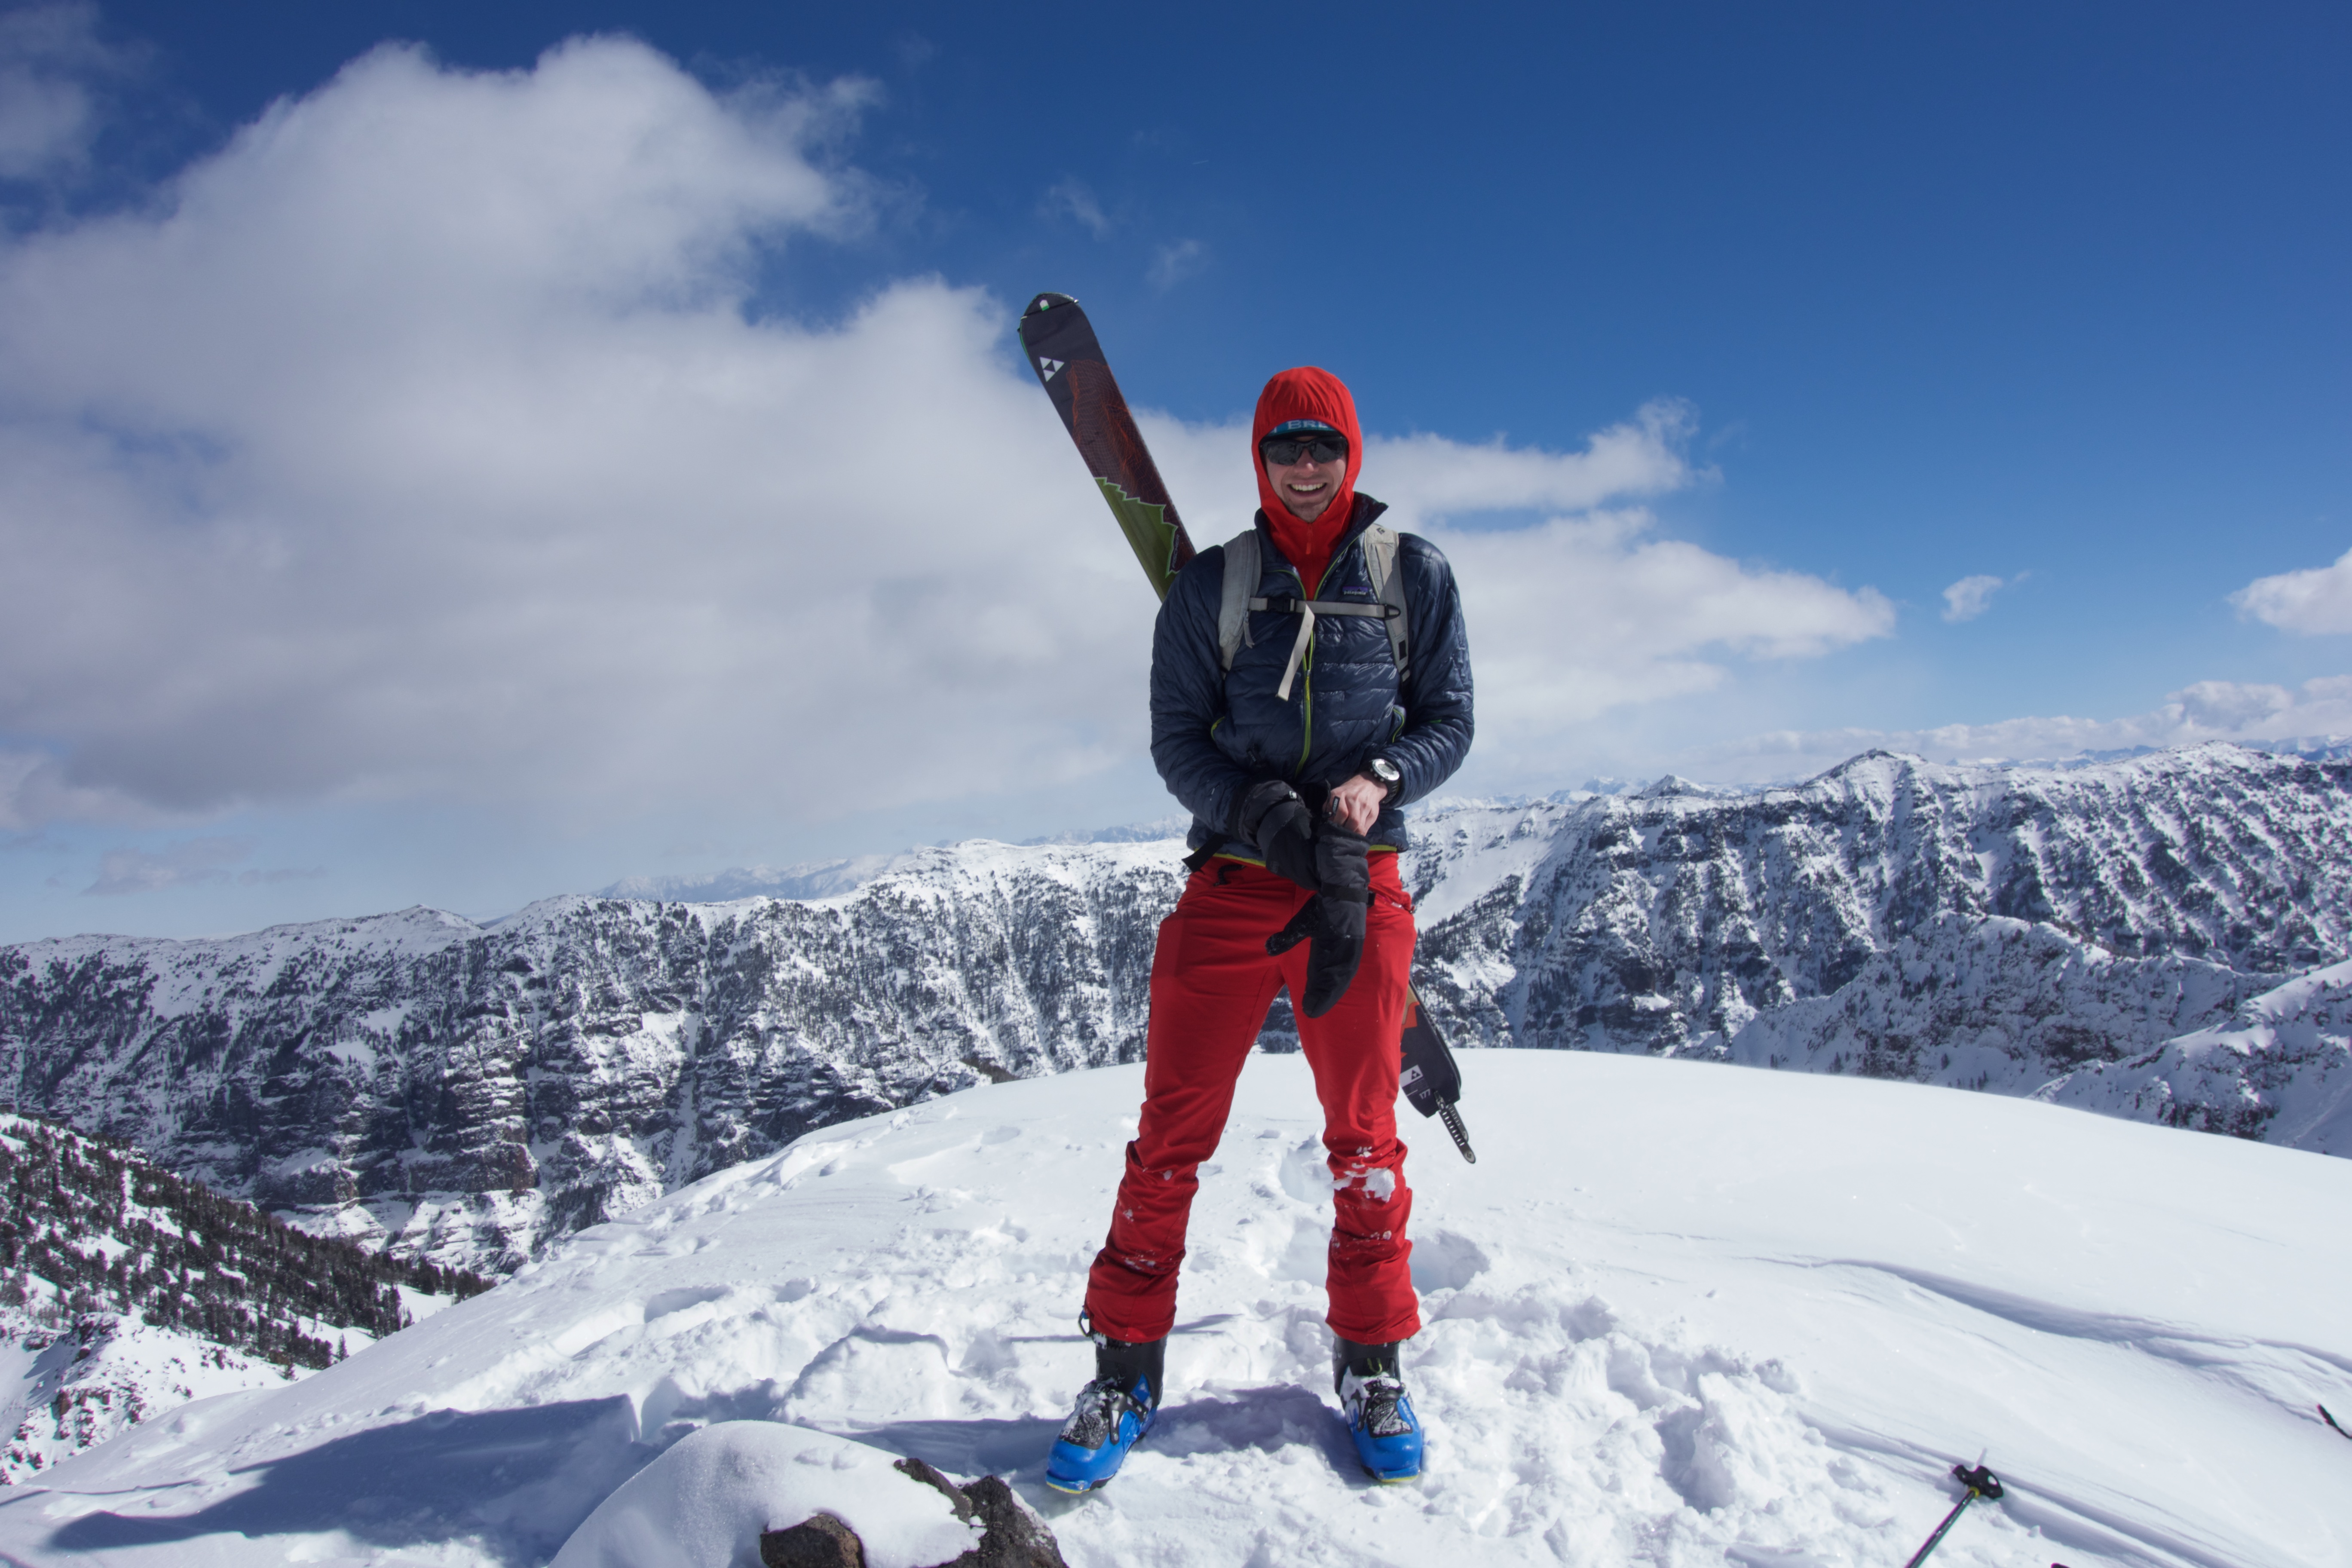
\includegraphics[height=30mm]{figs/sam-arden}
\end{block}
}

\frame{
    \frametitle{Persistence}
\begin{block}{Persistence Diagram}
\centering
	\only<1>{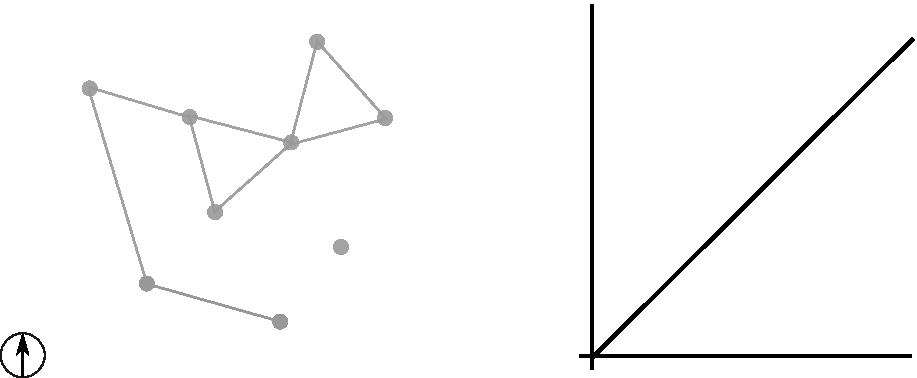
\includegraphics[width=\textwidth]{pdexampleOne}}%
	\only<2>{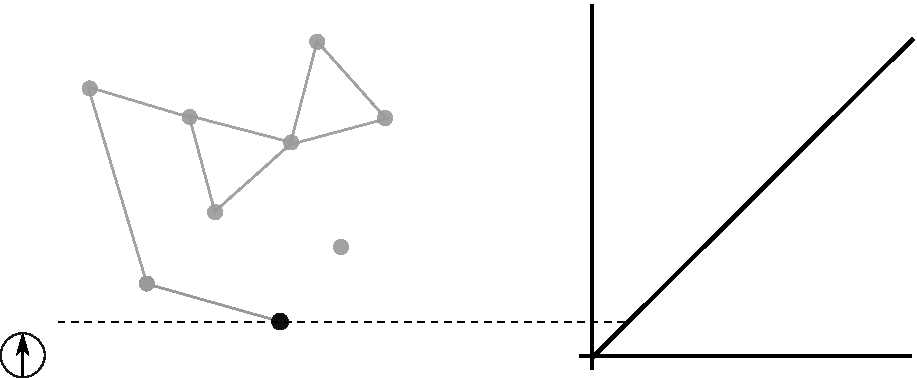
\includegraphics[width=\textwidth]{pdexampleTwo}}%
	\only<3>{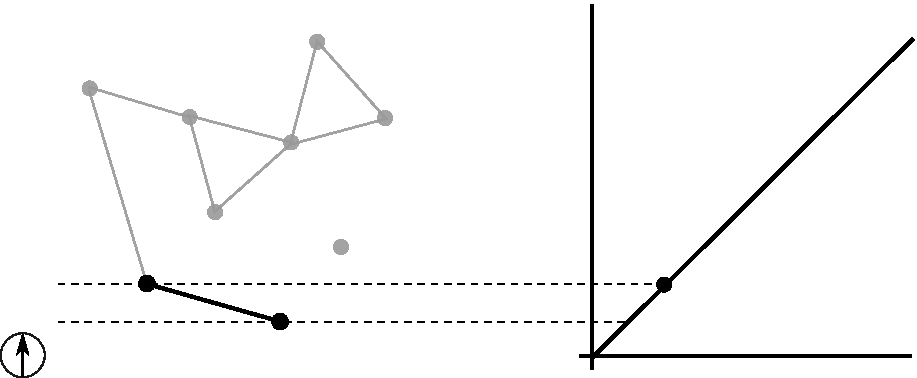
\includegraphics[width=\textwidth]{pdexampleThree}}%
	\only<4>{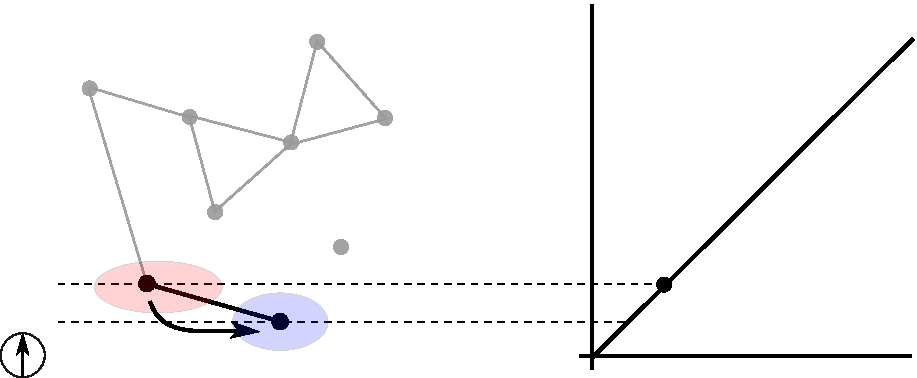
\includegraphics[width=\textwidth]{pdexampleFour}}%
	\only<5>{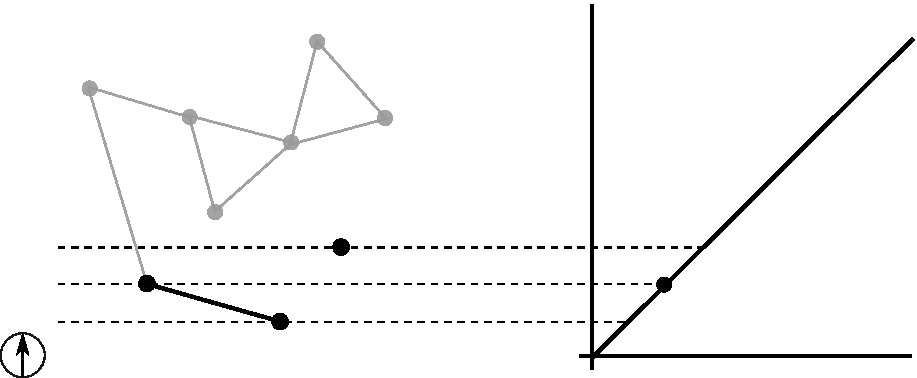
\includegraphics[width=\textwidth]{pdexampleFive}}%
	\only<6>{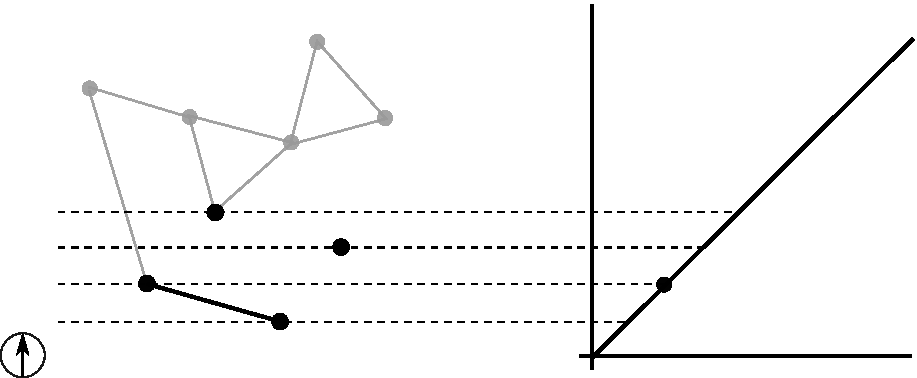
\includegraphics[width=\textwidth]{pdexampleSix}}%
	\only<7>{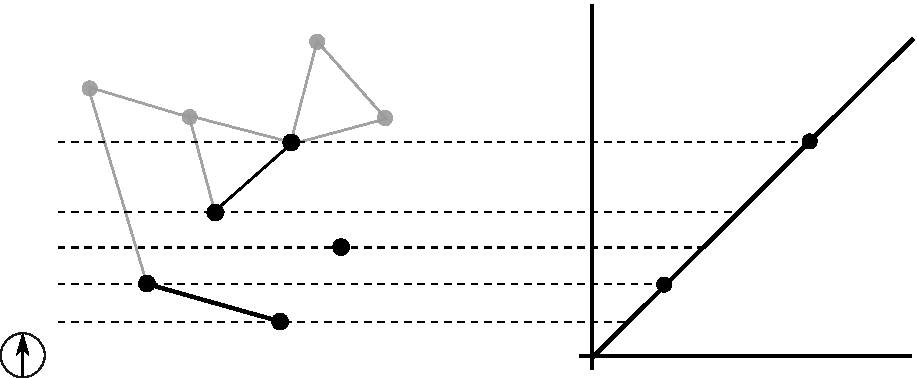
\includegraphics[width=\textwidth]{pdexampleSeven}}%
	\only<8>{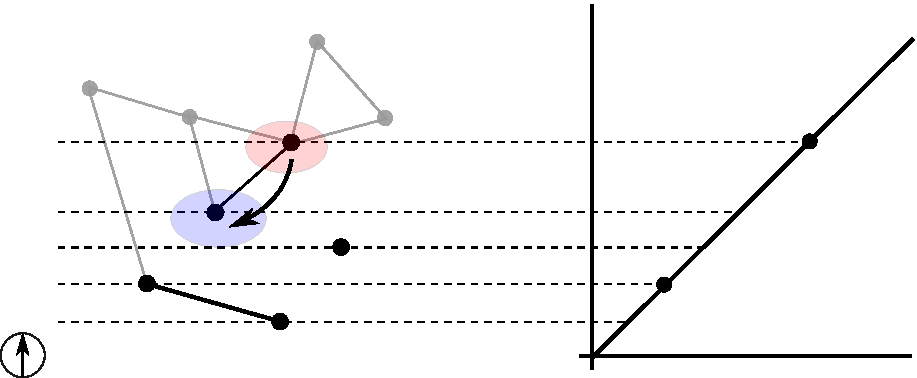
\includegraphics[width=\textwidth]{pdexampleEight}}%
	\only<9>{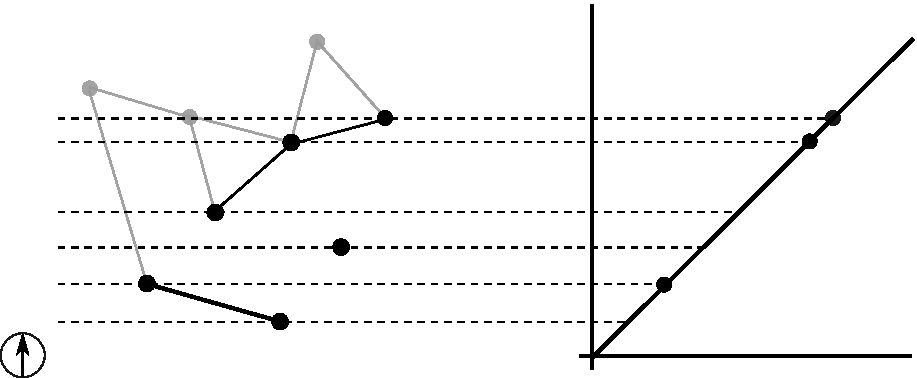
\includegraphics[width=\textwidth]{pdexampleNine}}%
	\only<10>{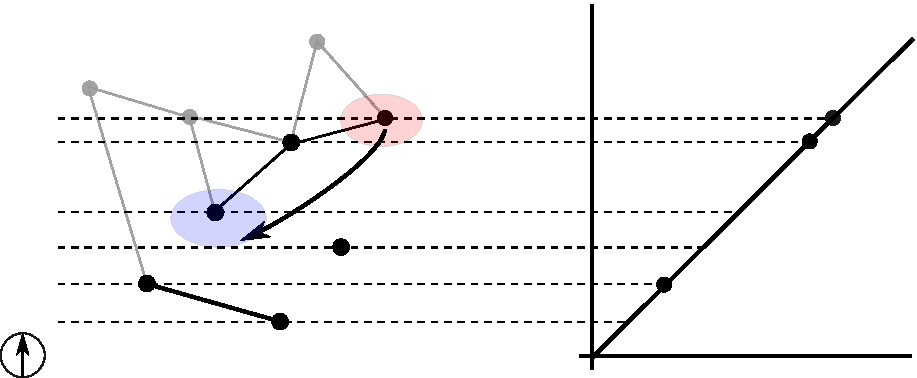
\includegraphics[width=\textwidth]{pdexampleTen}}%
	\only<11>{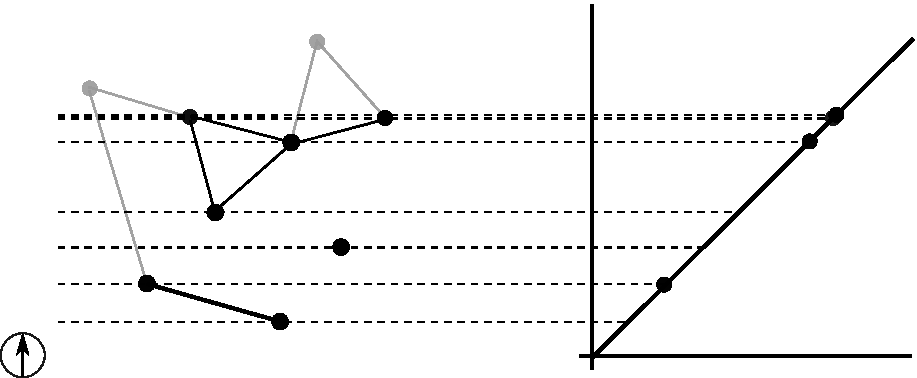
\includegraphics[width=\textwidth]{pdexampleEleven}}%
	\only<12>{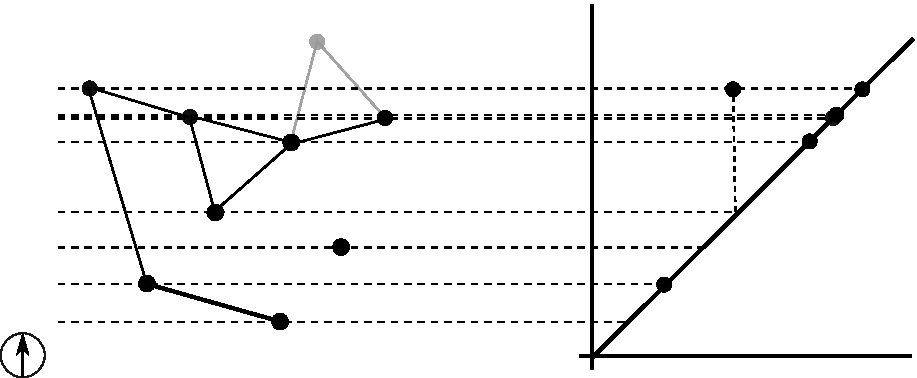
\includegraphics[width=\textwidth]{pdexampleTwelve}}%
	\only<13>{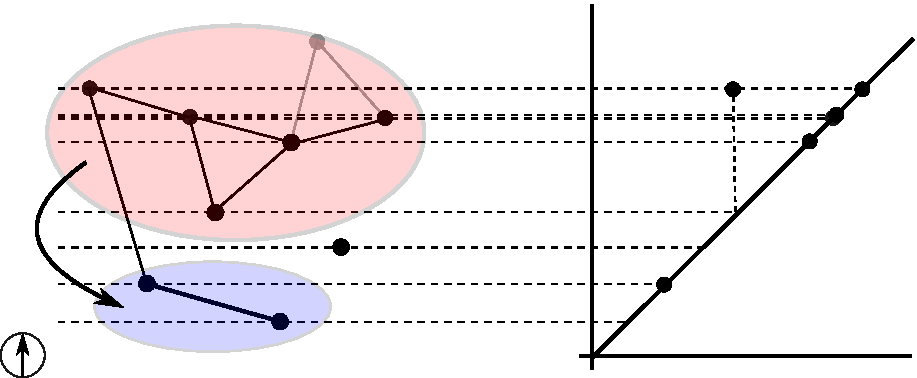
\includegraphics[width=\textwidth]{pdexampleThirteen}}%
	\only<14>{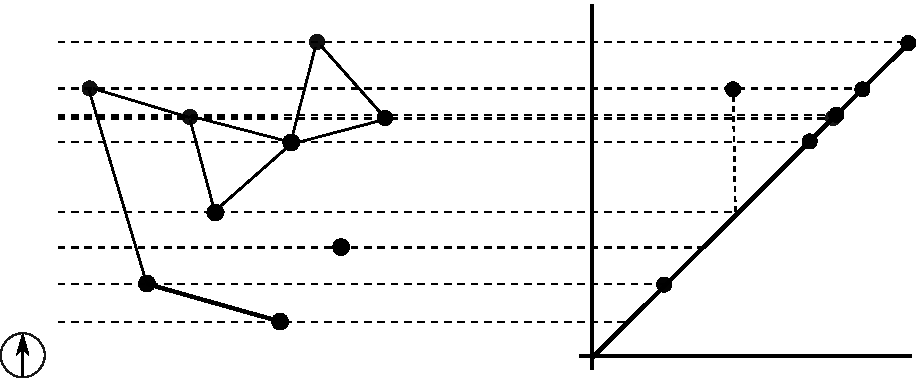
\includegraphics[width=\textwidth]{pdexampleFourteen}}%
	\only<15>{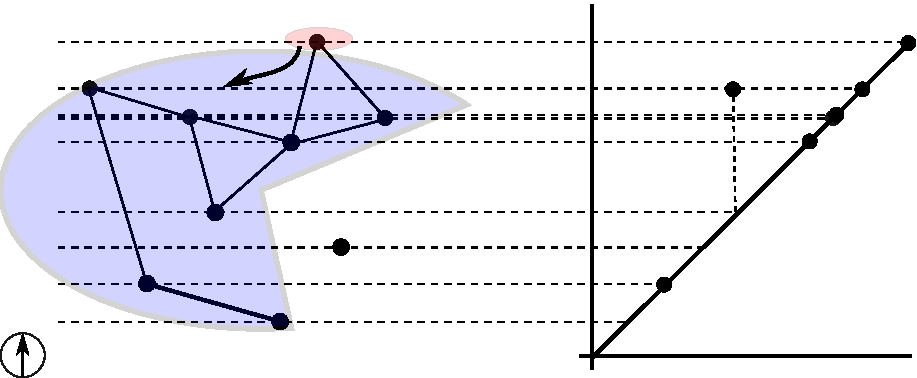
\includegraphics[width=\textwidth]{pdexampleFifteen}}%
	\only<16>{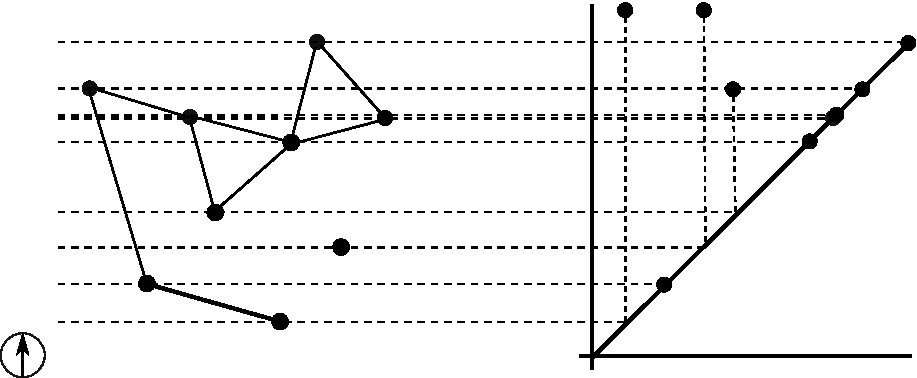
\includegraphics[width=\textwidth]{pdexampleSixteen}}%
	\vspace{5mm}%
    \newline
	\only<1->{\small{Intuition behind a degree zero persistence
	diagram.}}
\end{block}
}

\frame{
\frametitle{Comparing Two Persistence Diagrams}
\begin{block}{Bottleneck Distance}
\centering
    \only<1>{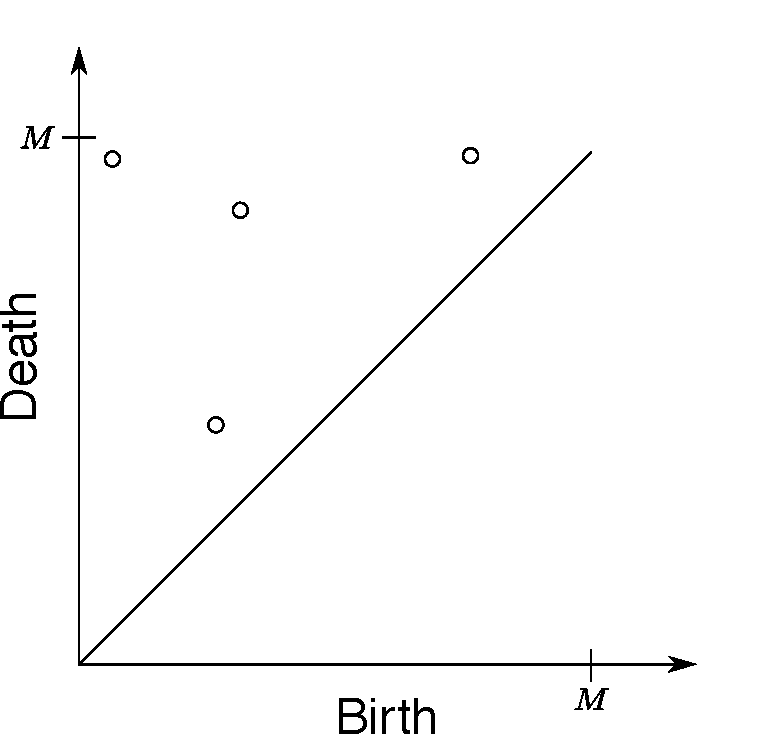
\includegraphics[width=.4\textwidth]{pdMatching1}}%
    \only<2>{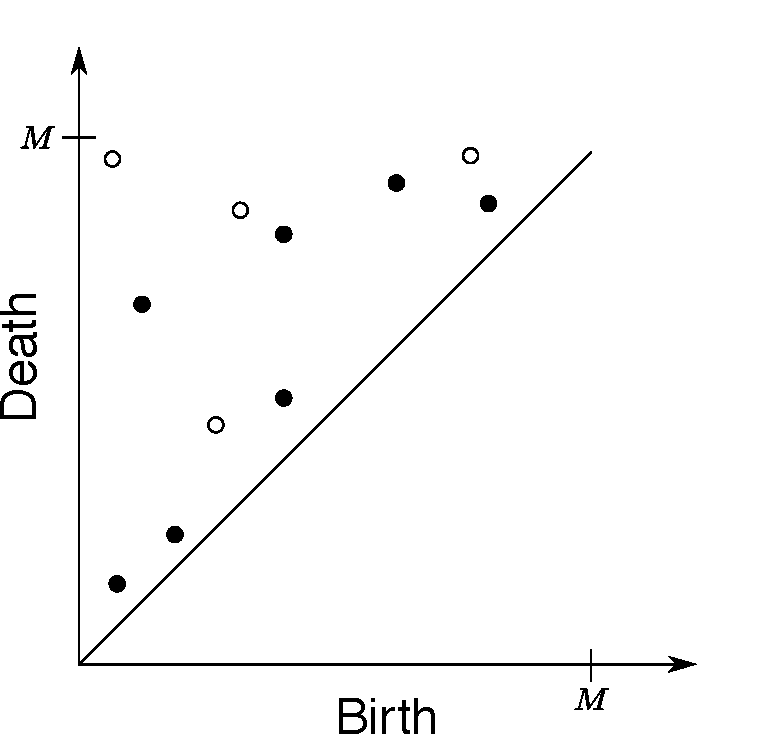
\includegraphics[width=.4\textwidth]{pdMatching2}}%
    \only<3>{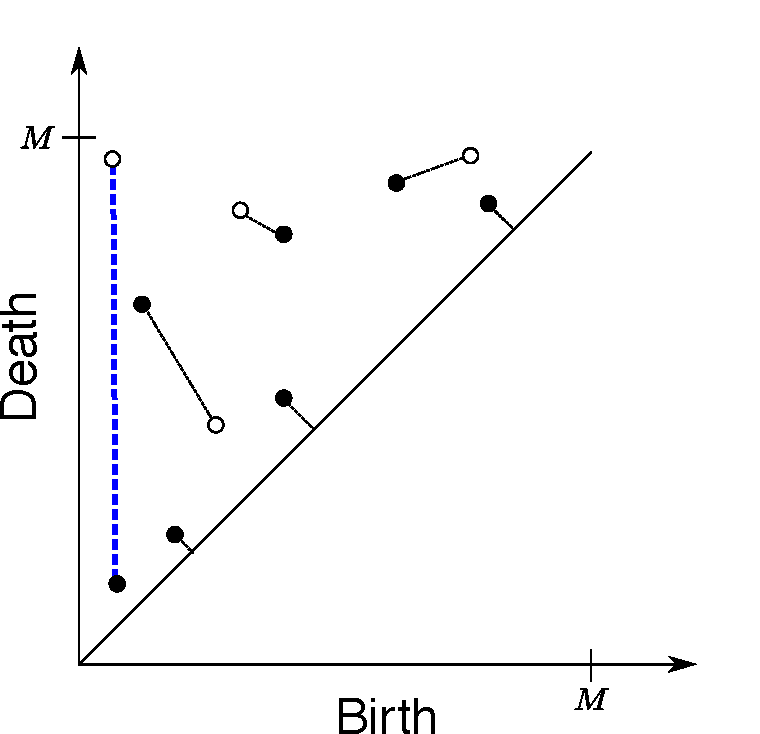
\includegraphics[width=.4\textwidth]{pdMatching3}}%
    \only<4>{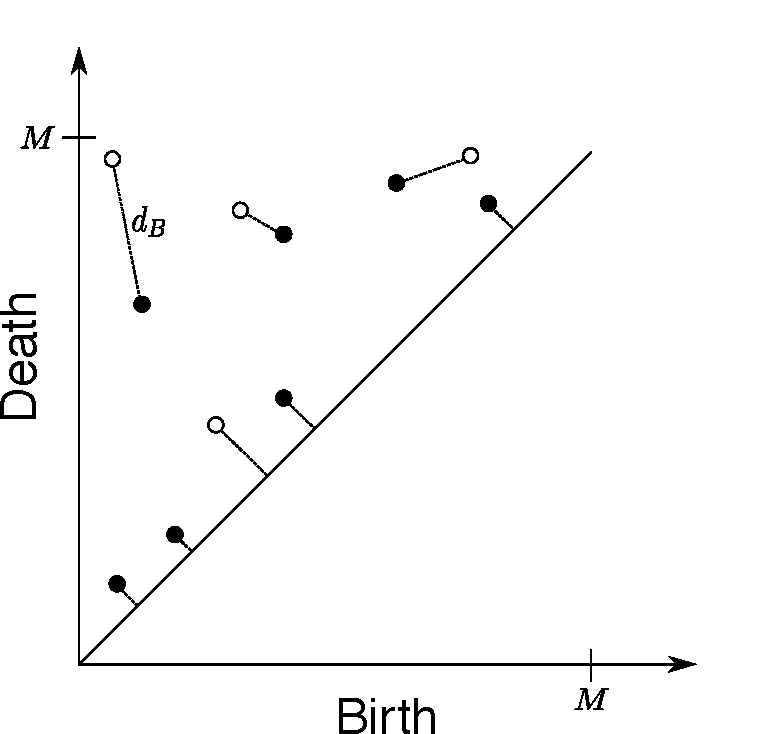
\includegraphics[width=.4\textwidth]{pdMatching4}}%
    \newline
    \emph{Bottleneck Distance}: is the minimum largest distance between two
    matched points over all matchings between two diagrams $P,Q$
    (matchings with diagonal allowed), denoted $d_B(P,Q)$.
\end{block}
}

\frame{
\frametitle{Querying Persistence Diagrams}
\begin{block}{Querying for Nearest Neighbor of Persistence Diagram}
\centering
    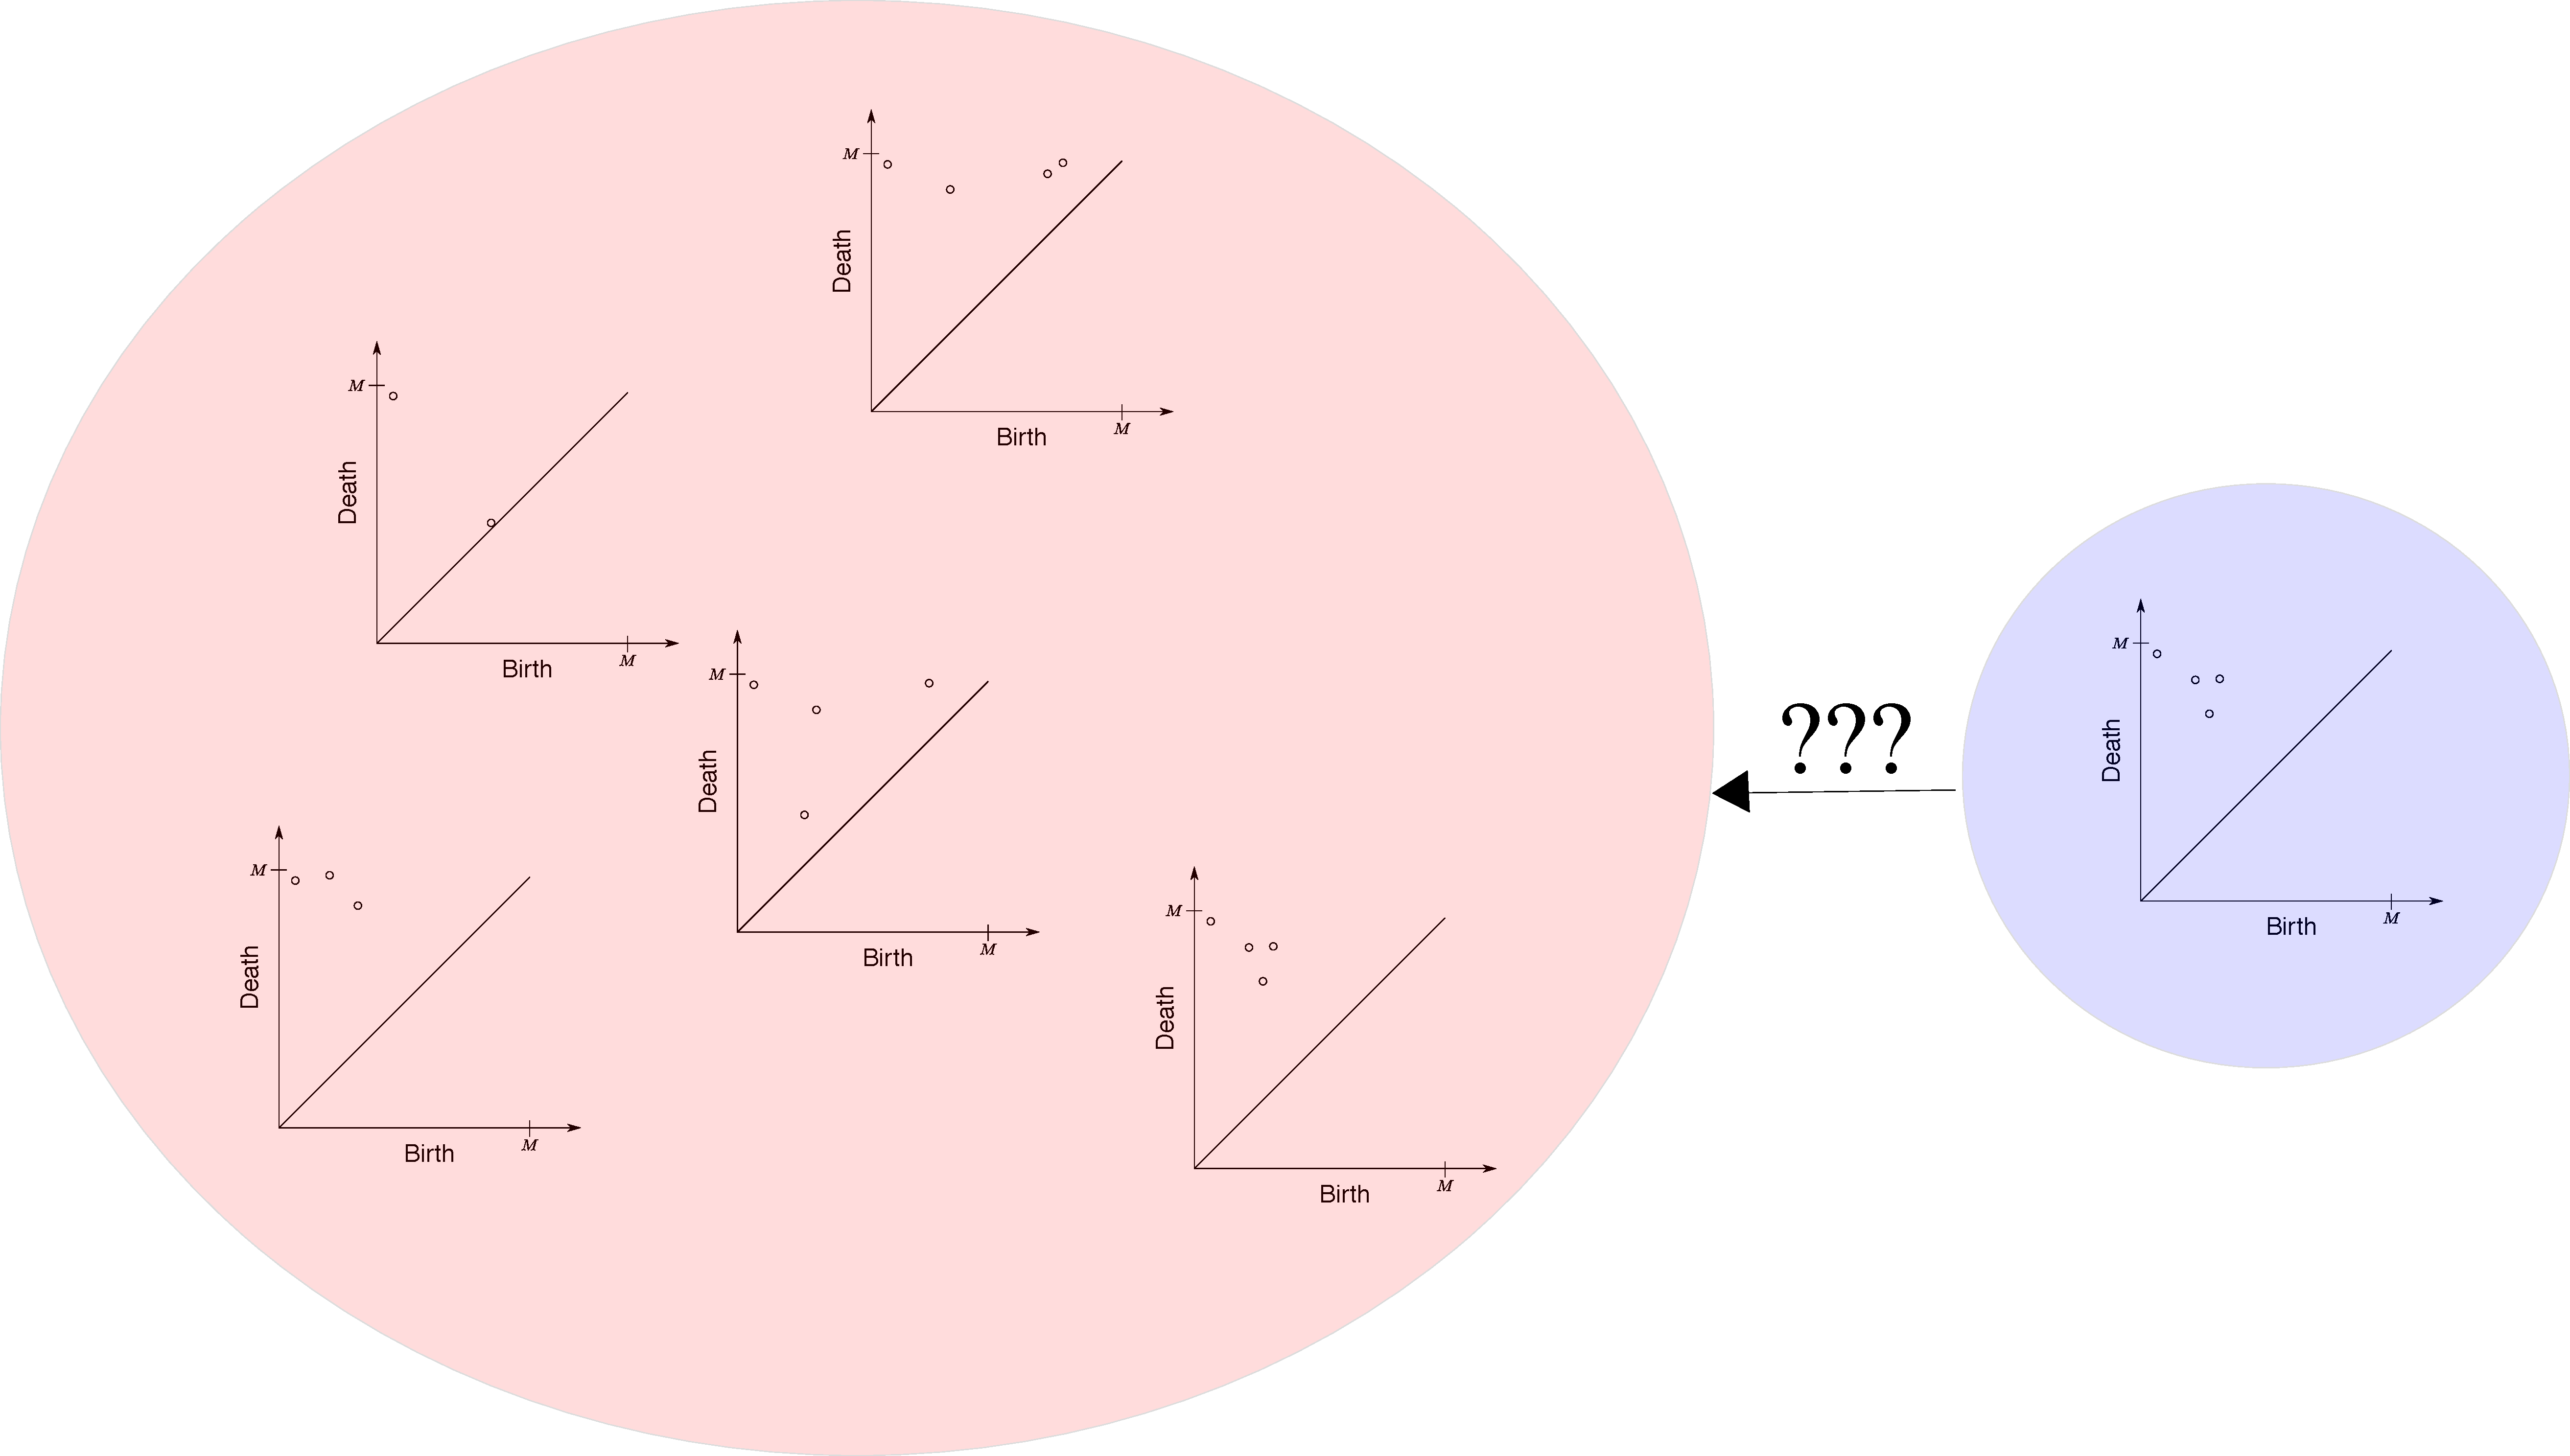
\includegraphics[width=.7\textwidth]{pdQuery}
\end{block}
}

\frame{
\frametitle{Searching in the Space of Persistence Diagrams}
\begin{block}{Project Information}
Brittany Terese Fasy, Xiaozhou He, Zhihui Liu, Samuel Micka, David L. Millman, Binhai Zhu, "Approximate Nearest Neighbors in the Space of Persistence Diagrams", (In Progress).

\centering
\vspace{5mm}
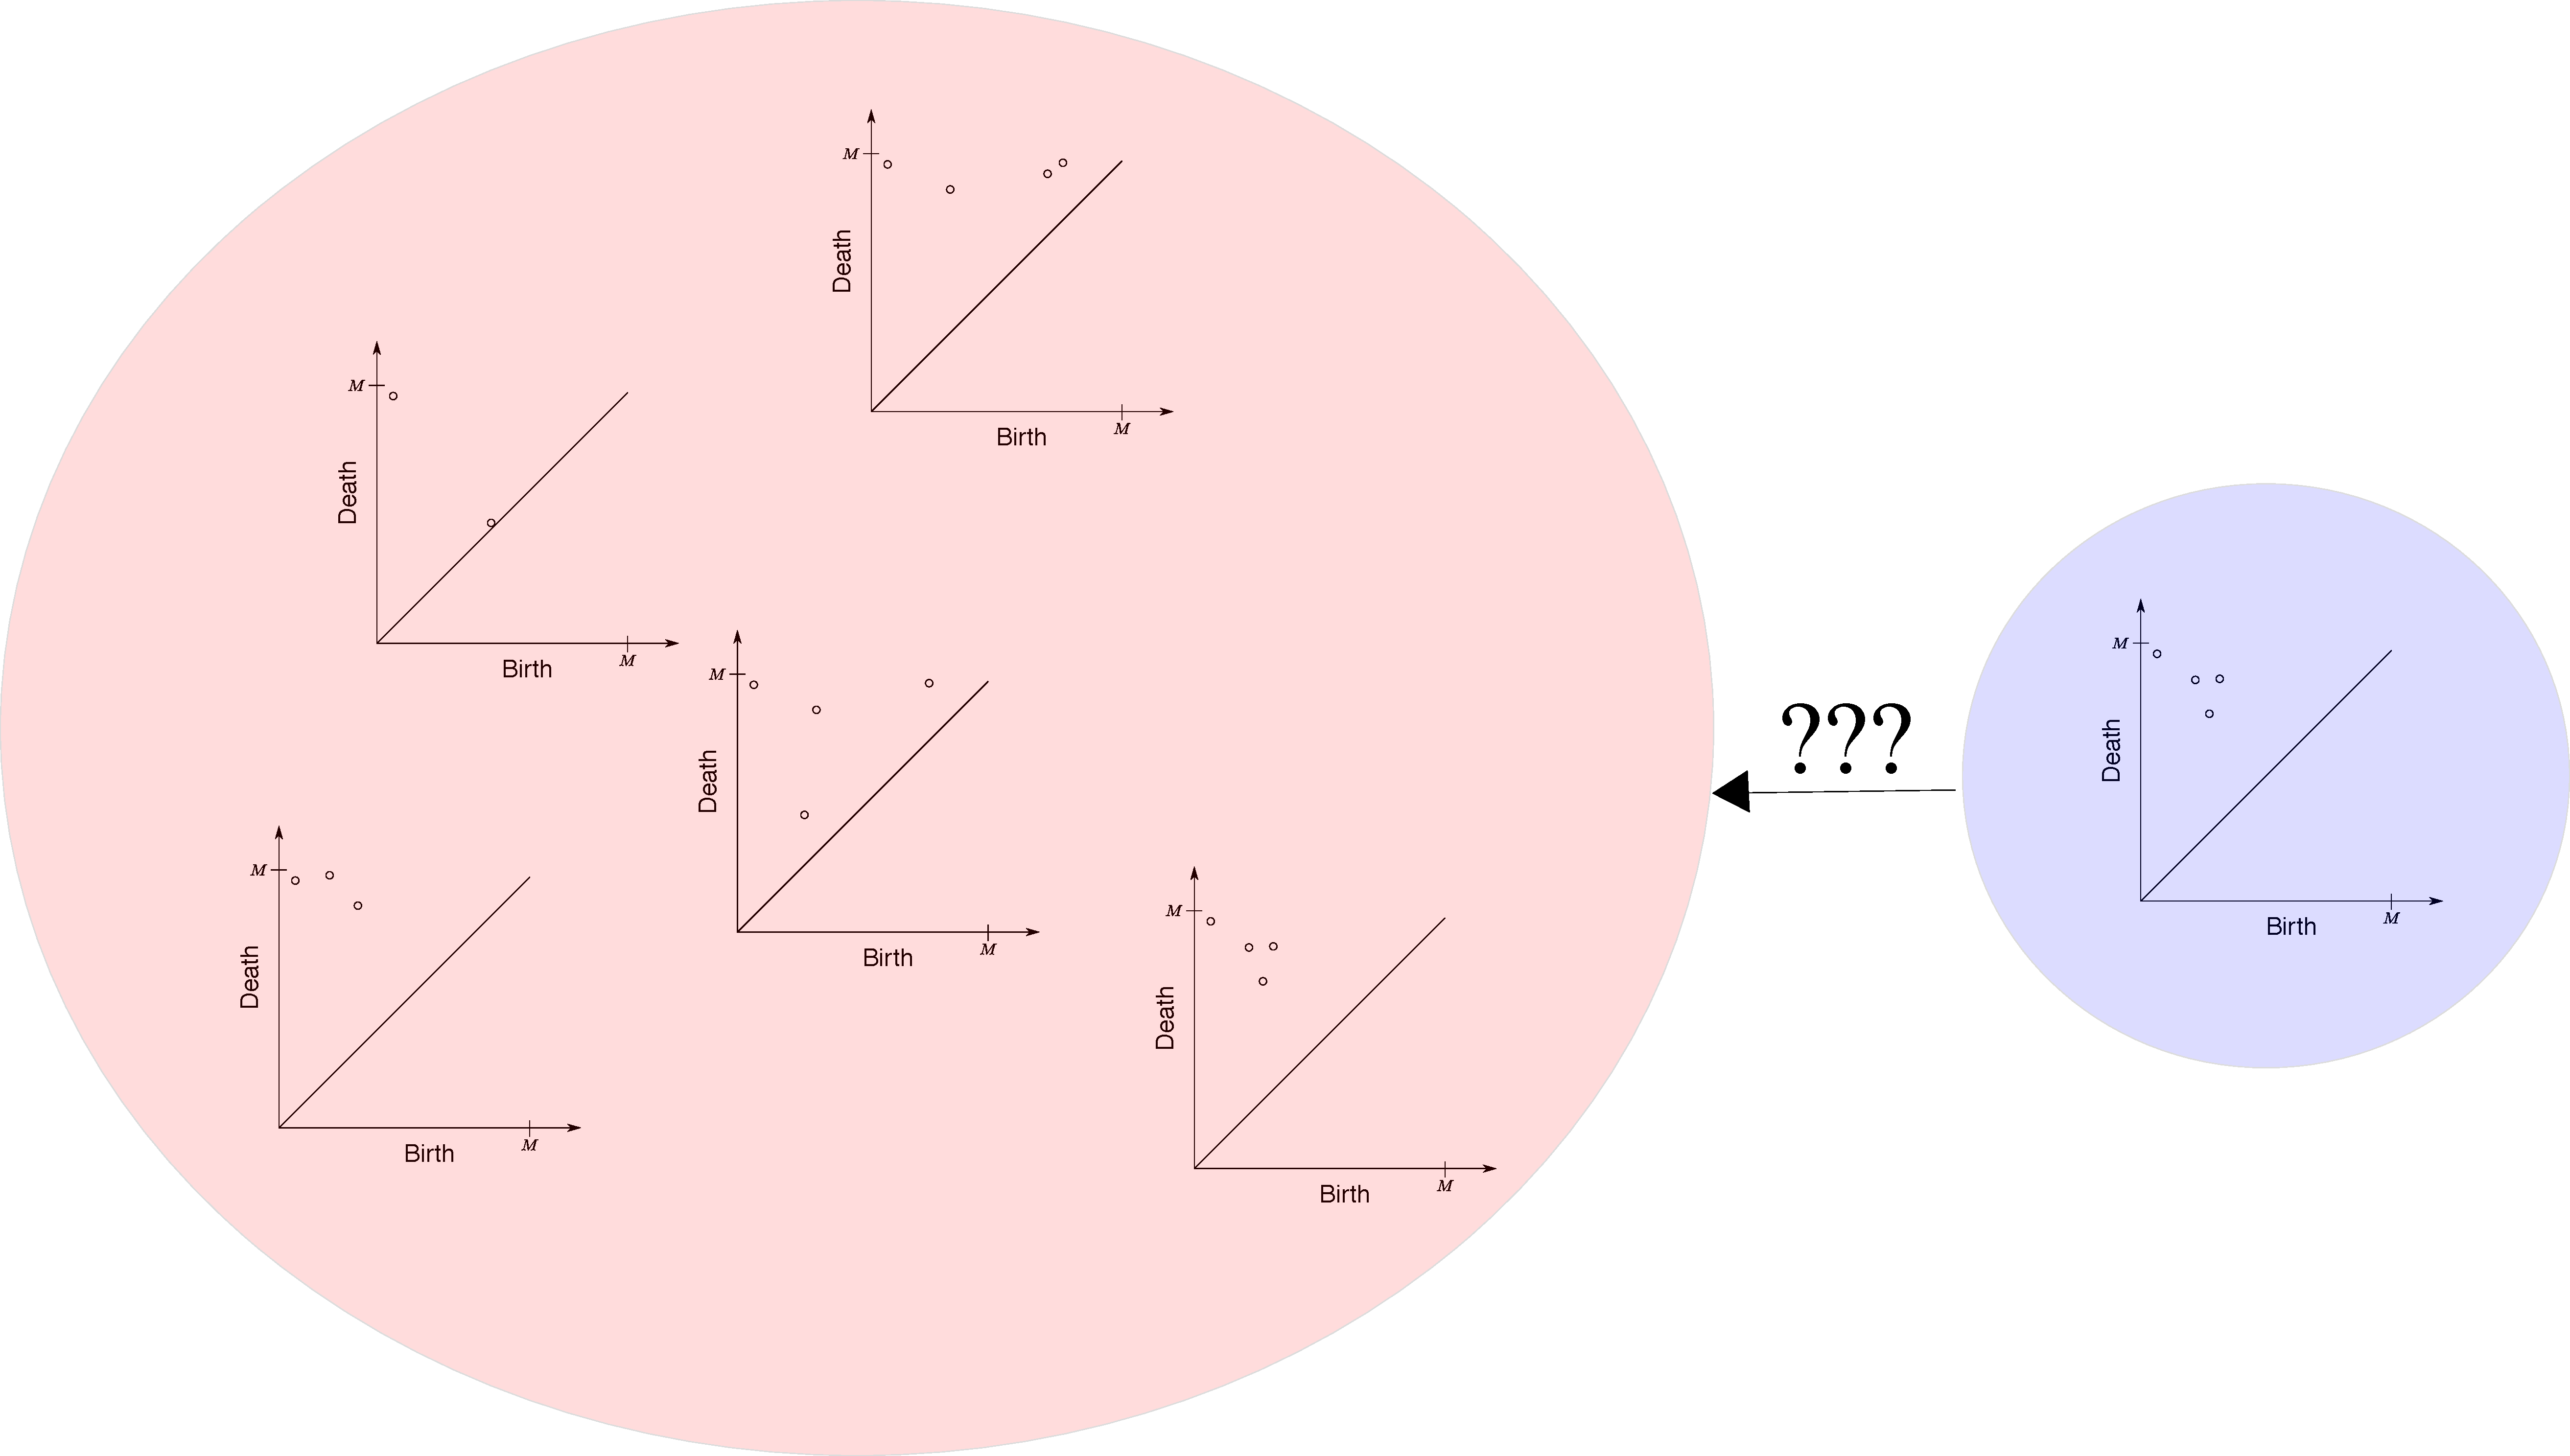
\includegraphics[width=.4\textwidth]{pdQuery}
\vspace{5mm}

Contact me at: samuelmicka@montana.edu

\end{block}
}

\end{document}
